\documentclass[tikz,border=10pt]{standalone}
\usepackage{amsmath} % For math environments and symbols

\begin{document}

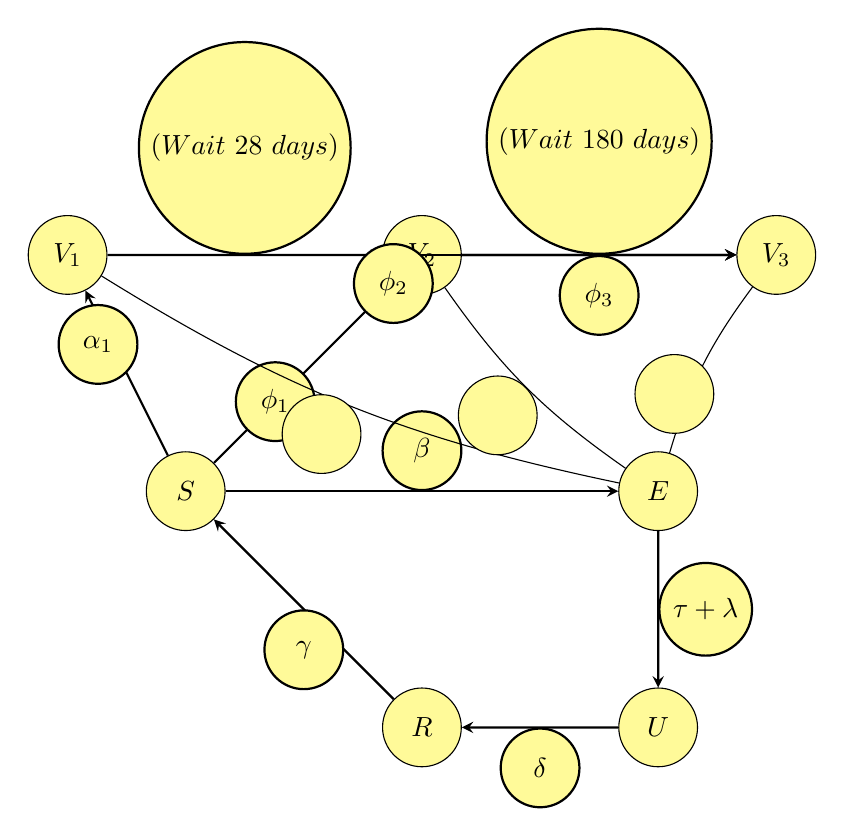
\begin{tikzpicture}[scale=1.5, every node/.style={circle, draw, fill=yellow!40, minimum size=1cm}]
    % Define nodes
    \node (S) at (0,0) {$S$};
    \node (E) at (4,0) {$E$};
    \node (U) at (4,-2) {$U$};
    \node (R) at (2,-2) {$R$};
    \node (V1) at (-1,2) {$V_1$};
    \node (V2) at (2,2) {$V_2$};
    \node (V3) at (5,2) {$V_3$};

    % Draw edges with labels
    \draw[-stealth, thick] (S) -- (V1) node [midway, above left] {$\alpha_1$};
    \draw[-stealth, thick] (S) -- (E) node [midway, above] {$\beta$};
    \draw[-stealth, thick] (E) -- (U) node [midway, right] {$\tau + \lambda$};
    \draw[-stealth, thick] (U) -- (R) node [midway, below] {$\delta$};
    \draw[-stealth, thick] (R) -- (S) node [midway, below] {$\gamma$};

    \draw[-stealth, thick] (V1) -- (V2) node [midway, above] {$(Wait~28~days)$};
    \draw[-stealth, thick] (V2) -- (V3) node [midway, above] {$(Wait~180~days)$};

    \draw[-stealth, thick] (S) -- (V2) node [midway, below left] {$\phi_1$};
    \draw[-stealth, thick] (V1) -- (V3) node [midway, below left] {$\phi_2$};
    \draw[-stealth, thick] (V2) -- (V3) node [midway, below] {$\phi_3$};

    % Add additional edge labels
    \path (V1) edge[bend right=10] node[midway, below left] {} (E);
    \path (V2) edge[bend right=10] node[midway, below left] {} (E);
    \path (V3) edge[bend right=10] node[midway, below left] {} (E);

\end{tikzpicture}

\end{document}